\documentclass{beamer}
 
 \usepackage[utf8x]{inputenc}
\usepackage[T1]{fontenc}
\usepackage[french]{babel}

\usepackage{lmodern, graphicx, tikz, pgfplots}
\usepackage{graphicx,amssymb,amstext,amsmath}
\usepackage{fancyhdr, url, ifthen, multirow}
\usepackage{subfig, float, caption}
\usepackage{array}
\usepackage{color, colortbl}
\usepackage{hyperref, siunitx}



\begin{document}

\title[Présentation]{Présentation Laboratoire}

\subtitle[\ldots]{}
\author{Groupe 11.64}
\institute[UCL]{Ecole polytechnique de Louvain}
\date{\today}
\maketitle

\begin{frame}
\frametitle{Interféromètre de Michelson}
\framesubtitle{Schéma}
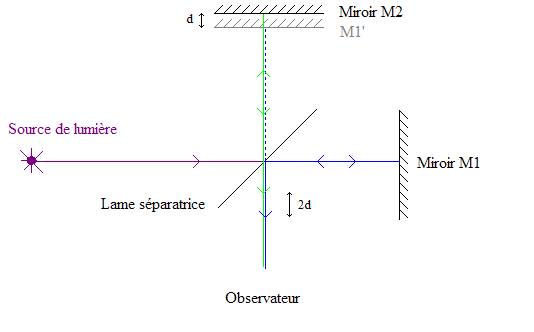
\includegraphics[scale=0.5]{schema.jpg}

$\Delta x = 1,2 cm$ $\rightarrow$  Ecart entre un minimum et un maximum 
$\lambda = 2,4 cm$


\end{frame} 

\begin{frame}
\frametitle{Interféromètre de Fabry-Pérot}
\framesubtitle{Schéma}
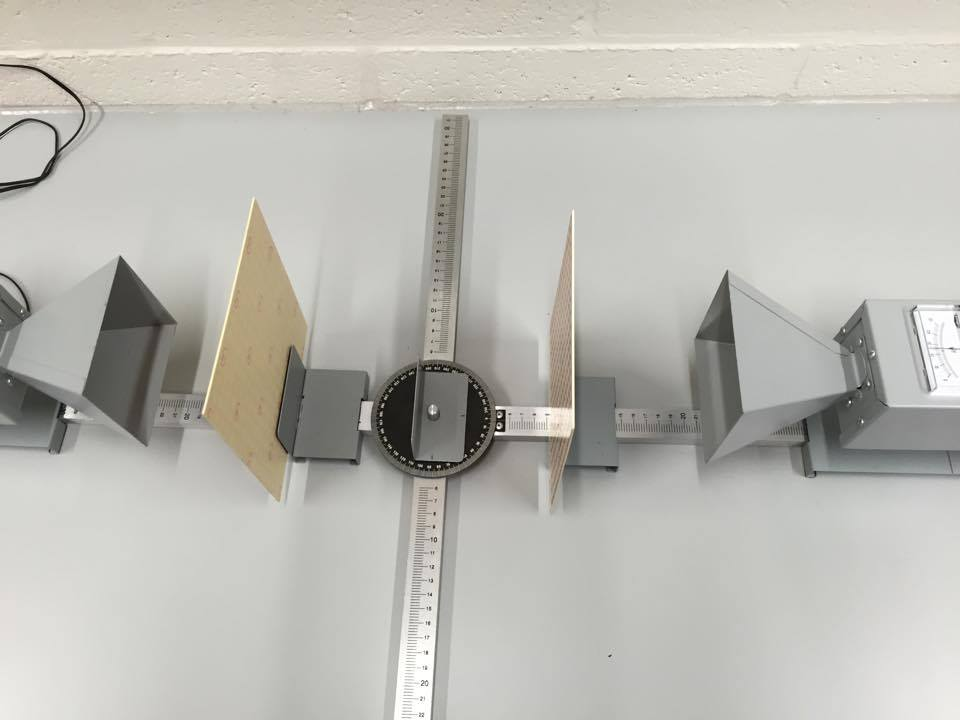
\includegraphics[scale=0.25]{schema1.jpg}

$\Delta x = 1,2 cm$ $\rightarrow$  Ecart entre un minimum et un maximum 
$\lambda = 2,4 cm$\\
Confirmation


\end{frame} 

\begin{frame}
\frametitle{Graphe diffraction}
\framesubtitle{Expérience avec les fentes}
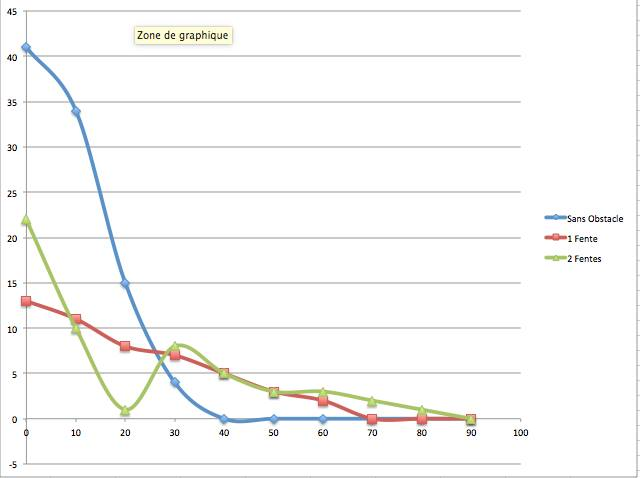
\includegraphics[scale=0.4]{schema2.jpg}

1 fente=diffraction;
2 fentes=diffraction+interférence


\end{frame} 



\end{document}
